%Physics: CoM, CoE, PE, Collisions, Momentum, KE
%Maths: 
\begin{hint}[HSC1950MIIIQ3l]
{A bullet of mass $m$ moving horizontally with velocity $u$ meets a block of wood of mass $M$ approaching with velocity $U$ and remains embedded in it.  Show that the loss of kinetic energy is
\begin{equation*}
 \frac{1}{2} \frac{Mm(u+U)^{2}}{M+m}.
\end{equation*}
} 
{Momentum, $\vtr{p} = m\vtr{v}$, is always conserved in collisions; the total before a collision equals the total after, taking care of the directions.}
{\textit{Used with permission from UCLES, Higher School Certificate Mathematics, June~1950, Paper~3, Question~3.}}
{The masses combine after impact, so there is only one unknown after the collision; this means conservation of momentum alone will give the final speed of the block. Drawing a diagram showing the system before and after the collisions, as in Figure \ref{fig:Dynamics_bullet_block}, always helps when solving a problem.

\begin{figure}[h]
	\centering
	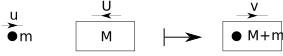
\includegraphics[width=0.6\textwidth]{Dynamics_bullet_block}
	\caption{}
	\label{fig:Dynamics_bullet_block}
\end{figure}

The two masses are moving in opposite directions, and since momentum is a vector quantity we must therefore subtract the momenta of $m$ and $M$ to find the total. Conservation of momentum then gives:
	\begin{align*} (m)(u) + (M)(-U) &= (M + m)(v) \\ mu - MU &= (M + m)v\end{align*}
and so the speed after the collision, $v$, is:
	\begin{equation*} v = \frac{mu - MU}{M + m} \end{equation*}

All that remains is to find the loss of kinetic energy in the collision; it involves a lot of tricky algebra, but nothing more:
\begin{align*} \textrm{KE loss} &= \textrm{KE}\s{initial} - \textrm{KE}\s{final} \\ \\
	&= \left[\frac{1}{2}mu^{2} + \frac{1}{2}MU^{2}\right] - \left[\frac{1}{2}(M + m)v^{2}\right] \\
	 &=  \left[\frac{1}{2}mu^{2} + \frac{1}{2}MU^{2}\right] - \left[\frac{1}{2}(M + m)\left(\frac{mu - MU}{M + m}\right)^{2}\right]
\end{align*} then expand out to cancel terms:

\begin{align*} \textrm{KE loss} &= \frac{1}{2}mu^{2} + \frac{1}{2}MU^{2} - \frac{1}{2(M + m)}\left(m^{2}u^{2} - 2MmuU + M^{2}U^{2}\right) \\ \\
	&= \frac{mu^{2}(M + m)}{2(M + m)} + \frac{MU^{2}(M + m)}{2(M + m)} - \frac{m^{2}u^{2}}{2(M + m)} + \frac{2MmuU}{2(M + m)} - \frac{M^{2}U^{2}}{2(M + m)} \\ \\
	&= \frac{1}{2(M + m)}\left[Mmu^{2} + \cancel{m^{2}u^{2}} + \cancel{M^{2}U^{2}} + mMU^{2} - \cancel{m^{2}u^{2}} - \cancel{M^{2}U^{2}} + 2MmuU\right] \\ \\
	&= \frac{Mm}{2(M + m)}\left[u^{2} + 2uU + U^{2}\right] \\ \\
	&= \frac{Mm(u + U)^{2}}{2(M + m)}
\end{align*} as required.
}
\end{hint}